\subsection{Modelo SIR} 
Este es un modelo clásico para epidemias, de nombre SIR, o Susceptibles. Infectados y Recuperados, creado por Kermack y McKendrick. 

Se basa en el uso de ecuaciones diferenciales ordinarias para describir una mecánica de contagios en una población cerrada de $N$ individuos susceptibles a contagiarse por el virus. A partir de un contagio inicial, este modelo describe el contagio a una determinada velocidad de infección $I$. Tras un periodo de tiempo, una persona infectada en este modelo, que no haya fallecido, se vuelve inmune al mismo; deja de recibir nuevas infecciones y pasa a ser catalogado como Recuperado $R$. Con forme pasa el tiempo en esta simulación, la población que es susceptible al contagio disminuye, hasta el punto en que esta deja de existir, resultando en una transformación total de la población inicial susceptible en población resistente y personas fallecidas.

El sustento del modelo SIR son un trio de ecuaciones diferenciales ordinarias descritas de la siguiente manera:

\begin{equation} \frac{dS}{dt} = -\beta S I \label{SIR_1} \end{equation}

Describe el cambio de personas susceptibles en un instante en concreto. Este siempre debe tender a un valor menor o igual a cero, pues se espera que conforme avance la epidemia, menos personas susceptibles queden, pues van siendo infectadas en el trascurso de esta.

\begin{equation} \frac{dI}{dt} = \beta S I - \nu I \label{SIR_2} \end{equation}

Representa cuantos nuevos infectados aparecen en un instante. Este valor siempre es mayor o igual a cero.

\begin{equation} \frac{dR}{dt} = \nu I \label{SIR_3} \end{equation}

Representa la cantidad de nuevos individuos resistentes a la infección en un instante.

Para que estas expresiones funcionen, los valores de la razón de transmición $ \beta > 0 $ y la taza de recuperación $ \nu > 0 $.
La Expresión $ \beta S I $ corresponde a la cantidad de nuevas infecciones en un determinado instante. Si reemplazamos la ecuación \eqref{SIR_3} en \eqref{SIR_2} podemos conseguir un valor para esta expresión en base a la derivada de Infectados y Recuperados tal que:

\begin{equation} \frac{dI}{dt} + \frac{dR}{dt} = \beta S I \end{equation}

La cual, a su vez, que posible reemplazar dentro de la ecuación \eqref{SIR_1}.

\begin{equation} \frac{dS}{dt} + \frac{dI}{dt} + \frac{dR}{dt} = 0 \end{equation}

Integrar esta última expresión nos da una expresión base para un modelo SIR que muestra uno de los problemas que contiene:

\begin{equation} S + I + R = Cte \end{equation}

El valor constante que se encontró con estas operaciones corresponde al numero $N$ del que se habló en un inicio. Como la población es cerrada, nunca cambia a lo largo del tiempo. El modelo SIR asume, además, que la epidemia presentada es relativamente breve en el tiempo. Tampoco ocurren nacimientos ni muertes naturales. No hay un periodo de infección latente, lo que implica que un individuo se vuelve infeccioso en el instante en que es infectado él mismo. La inmunidad que se obtiene del virus es permanente, y, el mayor problema, una mezcla en masa de individuos.

La mezcla en masa de individuos asume que la razón de encuentro entre la población susceptible e infectada es proporcional al producto de ambas poblaciones. Si se dobla la cantidad de cualquiera de estas resulta en el doble de infecciones en un instante de tiempo, lo cual es una suposición extraña. Un individuo en concreto solo mantiene contacto con una cantidad reducidad de otros individuos dentro de su propia comunidad.

Es natural razonar que la epidemia modelada por el Modelo SIR culmina en el tiempo cuando la cantidad de personas Susceptibles o la cantidad de personas infectadas llega a uno valor cero. Sin embargo, es posible comprobar que es imposible que el modelo SIR produzca una situación donde la población susceptible llegue a cero. Lo que modela la simulación es que, cuando ocurre un brote epidémico, la población susceptible decrese hasta un valor límite denotado por $S^\infty$. La población infectada, por otra parte, incrementa hasta un valor máximo, para luego decrecer hasta la extinción, comportamiento que pese a ser apto para la gran cantidad de epidemias que ha enfrentado la humanidad, se queda corto para el caso del COVID.

Este tipo de suposición poco razonables hace del modelo SIR uno poco útil para modelar la transmición del COVID-19. Sin embargo, aún es un punto inicial muy apto para la generación de otros modelos basados en éste.

\begin{figure}
    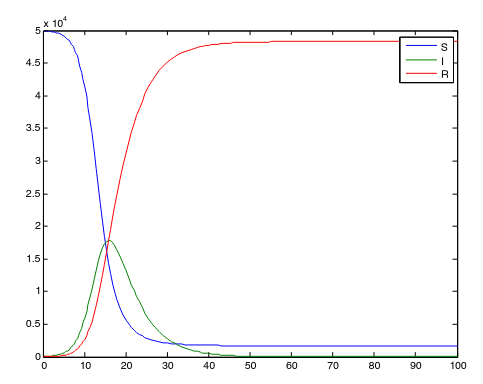
\includegraphics[width=\columnwidth]{Modelo SIR.png}
    \caption{Grafica de un Modelo SIR de un problema concreto \cite{weiss_2013}}
    \label{grafico modelo sir}
\end{figure}

En la figura \ref{grafico modelo sir} podemos apreciar una simulación calculada para un modelo matemático SIR determinado. Dentro de esta, podemos apreciar las tres ecuaciones que componen al modelo, y como estas cambiar a lo largo del tiempo.
